\section{Проблема у розв'язку задачі}

У даному підрозділі буде розглянута проблема
яке з першого погляду може здатися неочевидною,
проте стає досить явною при перегляді простих прикладів.

Задача, що розв'язується у згадуваних роботах,
може бути описана в загальному вигляді як
\begin{equation}\label{eq:argmin:improper}
  \left( k^*, \theta^* \right)
  = \argmin\limits_{k \in K, \theta \in \Theta}
    E\left( k, \theta \right),
\end{equation}
де $k$ --- набір параметрів, що є виходом алгоритму
(форма та, у більшості випадків, текстура),
$\theta$ --- набір параметрів,
що необхідні для генерації моделі, проте не є частиною виходу алгоритму
(матриця повороту, перспективи, переносу тощо).
Шукаються накращі $k^*$ і $\theta^*$,
а потім відкидається $\theta^*$ і вважається, що відповіддю є $k^*$.

Такий підхід може сдатися логічним.
Модель обличчя позиціонується максимально близько до того,
як розташоване реальне обличчя на пред'явленому зображенні.
Далі шукається найкраща форма (і текстура).
Вважається, що отримані значення є бажаним результатом,
бо немає сенсу робити так,
щоб на вихід впливали ті діляки зображення, на яких обличчя немає.
Проте звідки відомо, що обличчя насправді позиціоновано саме так,
як вказав алгоритм пошуку опорних точок?
Також немає гарантії, що тривимірні моделі були розмічені абсолютно точно.
Додаткову складність додає питання щодо кількості
і характеру опорних точок, які дадуть максимально точний результат.
Виникають такі ситуації,
коли одній конфігурації опорніх точок відповідає різне положення обличчя.
Простіший приклад: наявність проекції лише однієї опорної точки
не дає представлення щодо повороту та розміру обличчя.

Розглянемо конкретну ситуацію, коли підхід \eqref{eq:argmin:improper} є хибним.
На рис. \ref{fig:argmin:statue-original} зображено модель,
що була згенерована за допомогою BFM.
На рис. \ref{fig:argmin:statue-distorted} зображено ту ж саму модель,
проте до неї було застосовано матрицю перспективи.
Оскільки матриця перспективи --- аффінне перетворення, отже оборотне,
обидва зображення можуть грати роль як отриманого результату,
так і результату з іншою матрицею перспективи.
Нехай в кінці роботи алгоритму було отримано зображення
\ref{fig:argmin:statue-distorted} --- обличчя кремезної людини
з широким носом та вилицями і низьким лобом.
Слідуючи рекомендаціям,
ми зберігаємо лише параметри форми моделі та відкидаємо отриману матрицю.
В результаті маємо довгасте обличчя худої людини з високим лобом.

\begin{figure}[h]
  \centering
  \begin{subfigure}[b]{0.4\textwidth}
    \centering
    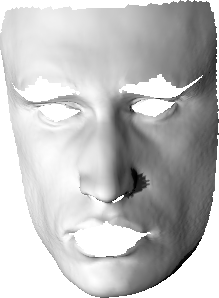
\includegraphics[width=\textwidth]{images/statue-orig}
    \caption{Визуалізована модель людського обличчя}
    \label{fig:argmin:statue-original}
  \end{subfigure}
  \begin{subfigure}[b]{0.4\textwidth}
    \centering
    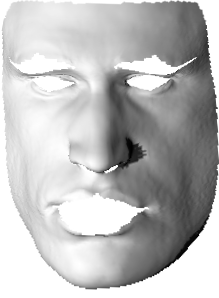
\includegraphics[width=\textwidth]{images/statue-perspective}
    \caption{Візуалізація з іншою матрицею перспективи}
    \label{fig:argmin:statue-distorted}
  \end{subfigure}
  \caption{Приклад візуалізації однієї моделі з різними параметрами камери}
\end{figure}

В такому випадку можна вирішити,
що перетворення, які з інтуїтивної точки зору змінюють зовнішній вигляд моделі
(масштаб, перспектива, скіс і таке інше),
можна зберігати разом із параметрами моделі як вихідний результат.
Проте не треба забувати, що ці перетворення були внесені в задачу,
щоб врахувати такі природні фактори,
як спотворення зображення різними об'єктивами фотокамер (зокрема перспектива).
Тому такий підхід теж є хибним.

У статті \cite{schlezinger:2013} було доведено,
що стратегія, яка використовує \eqref{eq:argmin:improper}, є негодящою,
бо можна знайти іншу стратегію,
яка буде давати кращі результати при будь-яких значеннях $\theta$.
